\definecolor{fftttt}{rgb}{1,0.2,0.2}
\definecolor{ttttff}{rgb}{0.2,0.2,1}
%dash pattern=on 5pt off 2pt
%[fill = white, rounded corners = 5pt, inner sep=0.8pt]
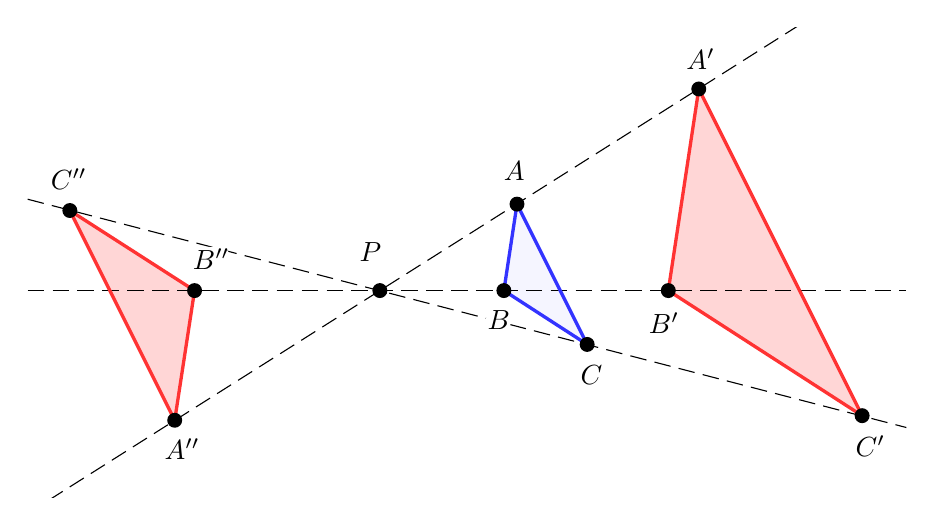
\begin{tikzpicture}[scale = 0.45]
    \clip(-7.57,-5.11) rectangle (17.23,8.14);
    \fill[color=ttttff,fill=ttttff,fill opacity=0.05] (6.24,3.16) -- (5.87,0.72) -- (8.22,-0.8) -- cycle;
    \fill[color=fftttt,fill=fftttt,fill opacity=0.2] (11.37,6.41) -- (10.51,0.72) -- (15.98,-2.81) -- cycle;
    \fill[color=fftttt,fill=fftttt,fill opacity=0.2] (-3.42,-2.94) -- (-2.86,0.72) -- (-6.38,2.98) -- cycle;
    \draw [dash pattern=on 6pt off 3pt,domain=-7.57:17.23] plot(\x,{(--2.51-0*\x)/3.5});
    \draw [dash pattern=on 6pt off 3pt,domain=-7.57:17.23] plot(\x,{(-3.02--2.45*\x)/3.87});
    \draw [dash pattern=on 6pt off 3pt,domain=-7.57:17.23] plot(\x,{(--7.79-1.52*\x)/5.85});
    \draw [line width=1.2pt,color=ttttff] (6.24,3.16)-- (5.87,0.72);
    \draw [line width=1.2pt,color=ttttff] (5.87,0.72)-- (8.22,-0.8);
    \draw [line width=1.2pt,color=ttttff] (8.22,-0.8)-- (6.24,3.16);
    \draw [line width=1.2pt,color=fftttt] (11.37,6.41)-- (10.51,0.72);
    \draw [line width=1.2pt,color=fftttt] (10.51,0.72)-- (15.98,-2.81);
    \draw [line width=1.2pt,color=fftttt] (15.98,-2.81)-- (11.37,6.41);
    \draw [line width=1.2pt,color=fftttt] (-3.42,-2.94)-- (-2.86,0.72);
    \draw [line width=1.2pt,color=fftttt] (-2.86,0.72)-- (-6.38,2.98);
    \draw [line width=1.2pt,color=fftttt] (-6.38,2.98)-- (-3.42,-2.94);
    \begin{scriptsize}
        \normalsize
        \fill [color=black] (2.37,0.72) circle (6.0pt);
        \draw[color=black] (2.1,1.81) node[fill = white, rounded corners = 5pt, inner sep=0.8pt] {$P$};
        \fill [color=black] (6.24,3.16) circle (6.0pt);
        \draw[color=black] (6.16,4.08) node[fill = white, rounded corners = 5pt, inner sep=0.8pt] {$A$};
        \fill [color=black] (5.87,0.72) circle (6.0pt);
        \draw[color=black] (5.73,-0.11) node[fill = white, rounded corners = 5pt, inner sep=0.8pt] {$B$};
        \fill [color=black] (8.22,-0.8) circle (6.0pt);
        \draw[color=black] (8.34,-1.65) node[fill = white, rounded corners = 5pt, inner sep=0.8pt] {$C$};
        \fill [color=black] (10.51,0.72) circle (6.0pt);
        \draw[color=black] (10.39,-0.2) node[fill = white, rounded corners = 5pt, inner sep=0.8pt] {$B'$};
        \fill [color=black] (-2.86,0.72) circle (6.0pt);
        \draw[color=black] (-2.39,1.6) node[fill = white, rounded corners = 5pt, inner sep=0.8pt] {$B''$};
        \fill [color=black] (11.37,6.41) circle (6.0pt);
        \draw[color=black] (11.42,7.24) node[fill = white, rounded corners = 5pt, inner sep=0.8pt] {$A'$};
        \fill [color=black] (15.98,-2.81) circle (6.0pt);
        \draw[color=black] (16.21,-3.66) node[fill = white, rounded corners = 5pt, inner sep=0.8pt] {$C'$};
        \fill [color=black] (-3.42,-2.94) circle (6.0pt);
        \draw[color=black] (-3.21,-3.75) node[fill = white, rounded corners = 5pt, inner sep=0.8pt] {$A''$};
        \fill [color=black] (-6.38,2.98) circle (6.0pt);
        \draw[color=black] (-6.41,3.86) node[fill = white, rounded corners = 5pt, inner sep=0.8pt] {$C''$};
    \end{scriptsize}
\end{tikzpicture}